\documentclass[a4paper]{article}
\usepackage{amsmath,amssymb,caption,float,graphicx,indentfirst,parskip,tabularx,xcolor}
% \usepackage{hyperref}
% \usepackage{minted}
% \usepackage[utf8]{inputenc}
% \usepackage[english]{babel}
% \usepackage[backend=bibtex]{biblatex}
% \addbibresource{Lab3.bib}
\captionsetup[figure]{labelsep=period}
% \captionsetup[listing]{labelsep=period}
% \definecolor{bg}{rgb}{0.95,0.95,0.95}
% \hypersetup{colorlinks=true,linkcolor=blue,filecolor=blue,urlcolor=blue,citecolor=cyan}
\setlength{\parindent}{2em}
% \usemintedstyle{emacs}
\begin{document}
\begin{titlepage}
    \vspace*{0.25cm}
    \noindent\rule[0.25\baselineskip]{\textwidth}{1pt}
    \begin{center}
        \huge{\textsc{UM--SJTU Joint Institute}}\vspace{0.3em}\\
        \huge{\textbf{System-on-Chip Design (ECE4810J)}}\vspace{0.3em}\\
        \noindent\rule[0.25\baselineskip]{\textwidth}{1pt}
    \end{center}
    \begin{center}
        \vspace{5cm}
        \Large{\textsc{Laboratory Report}}\vspace{0.5em}\\
        \Large{\textbf{Lab 6. Getting Started with the OpenLane ASIC Design Flow and Skywater 130nm Technology}}\vspace{1em}\\
        \Large{\textbf{Group 2}}\\
    \end{center}
    \vfill
    \large
    \begin{tabular}{ll}
        Name: Haochen Wu \hspace*{2em}&ID: 518021910558\hspace*{2em}\\
        Name: Siyuan Zhang \hspace*{2em}&ID: 518370910180 \hspace*{2em}\\
        Name: Yihua Liu \hspace*{2em}&ID: 518021910998\hspace*{2em}\\
        \\
        Date: November 19, 2021
    \end{tabular}
\end{titlepage}
\tableofcontents
\newpage
\section{Overview}
In this lab, we will get familiarised with the TCL(“Tool Command Language”) script language grammar and OpenLane VLSI design flow together with Skywater 130nm PDK. OpenLane is an open-source VLSI flow built around open-source tools,
where a collection of scripts that run these tools gather in the right order and transform their inputs
and outputs appropriately.

\section{TCL}
TCL (“Tool Command Language”) is a shell script language that is widely used in most digital design flows nowadays.
\subsection{Problem 1}
Write a procedure (proc) called “avg” that takes an array of numbers with any length and return the average of it.

Code: 
\begin{figure}[H]
    \centering
    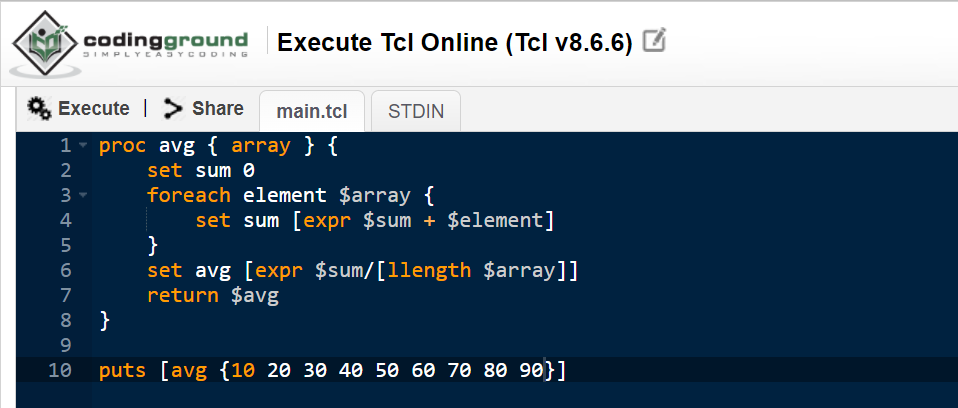
\includegraphics[width=1\textwidth]{part2_1_code.png}
    \caption{Code screenshot of problem 1.}
\end{figure}
Running result:
\begin{figure}[H]
    \centering
    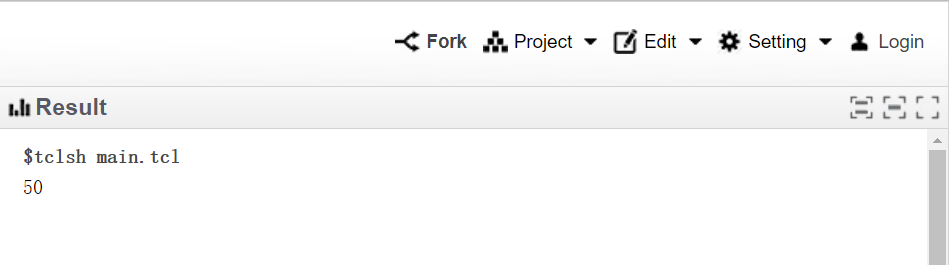
\includegraphics[width=1\textwidth]{part2_1_result.png}
    \caption{Result screenshot of problem 1.}
\end{figure}
Here we can see this function gives the output of 50, which is the average of set {10, 20, 30, 40, 50, 60, 70, 80, 90}. This TCL script works properly. 

\subsection{Problem 2}
Write a procedure (proc) that does the factorial function.

Code: 
\begin{figure}[H]
    \centering
    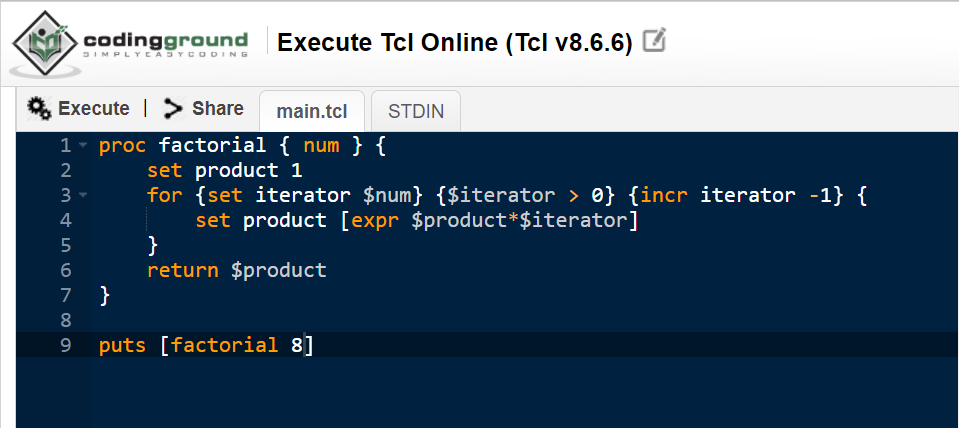
\includegraphics[width=1\textwidth]{part2_2_code.png}
    \caption{Code screenshot of problem 2.}
\end{figure}
Running result:
\begin{figure}[H]
    \centering
    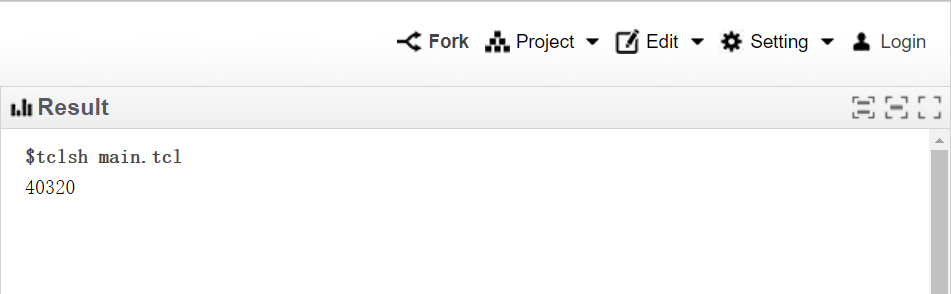
\includegraphics[width=1\textwidth]{part2_2_result.png}
    \caption{Result screenshot of problem 2.}
\end{figure}
This function gives the output of 40320, which is the factorial product of 8*7*6*5*4*3*2*1 = 40320. This TCL script works properly.

\section{Setting up the OpenLane flow}
\subsection{Displaying the Final Layout(3.4 in lab manual)}
Here we run the design of "spm" through the flow and obtain the results in corresponding "magic" and "klayout" folder. We use "Klayout" to see these generated layout file.

For "spm.gdc" in "magic" folder:
\begin{figure}[H]
    \centering
    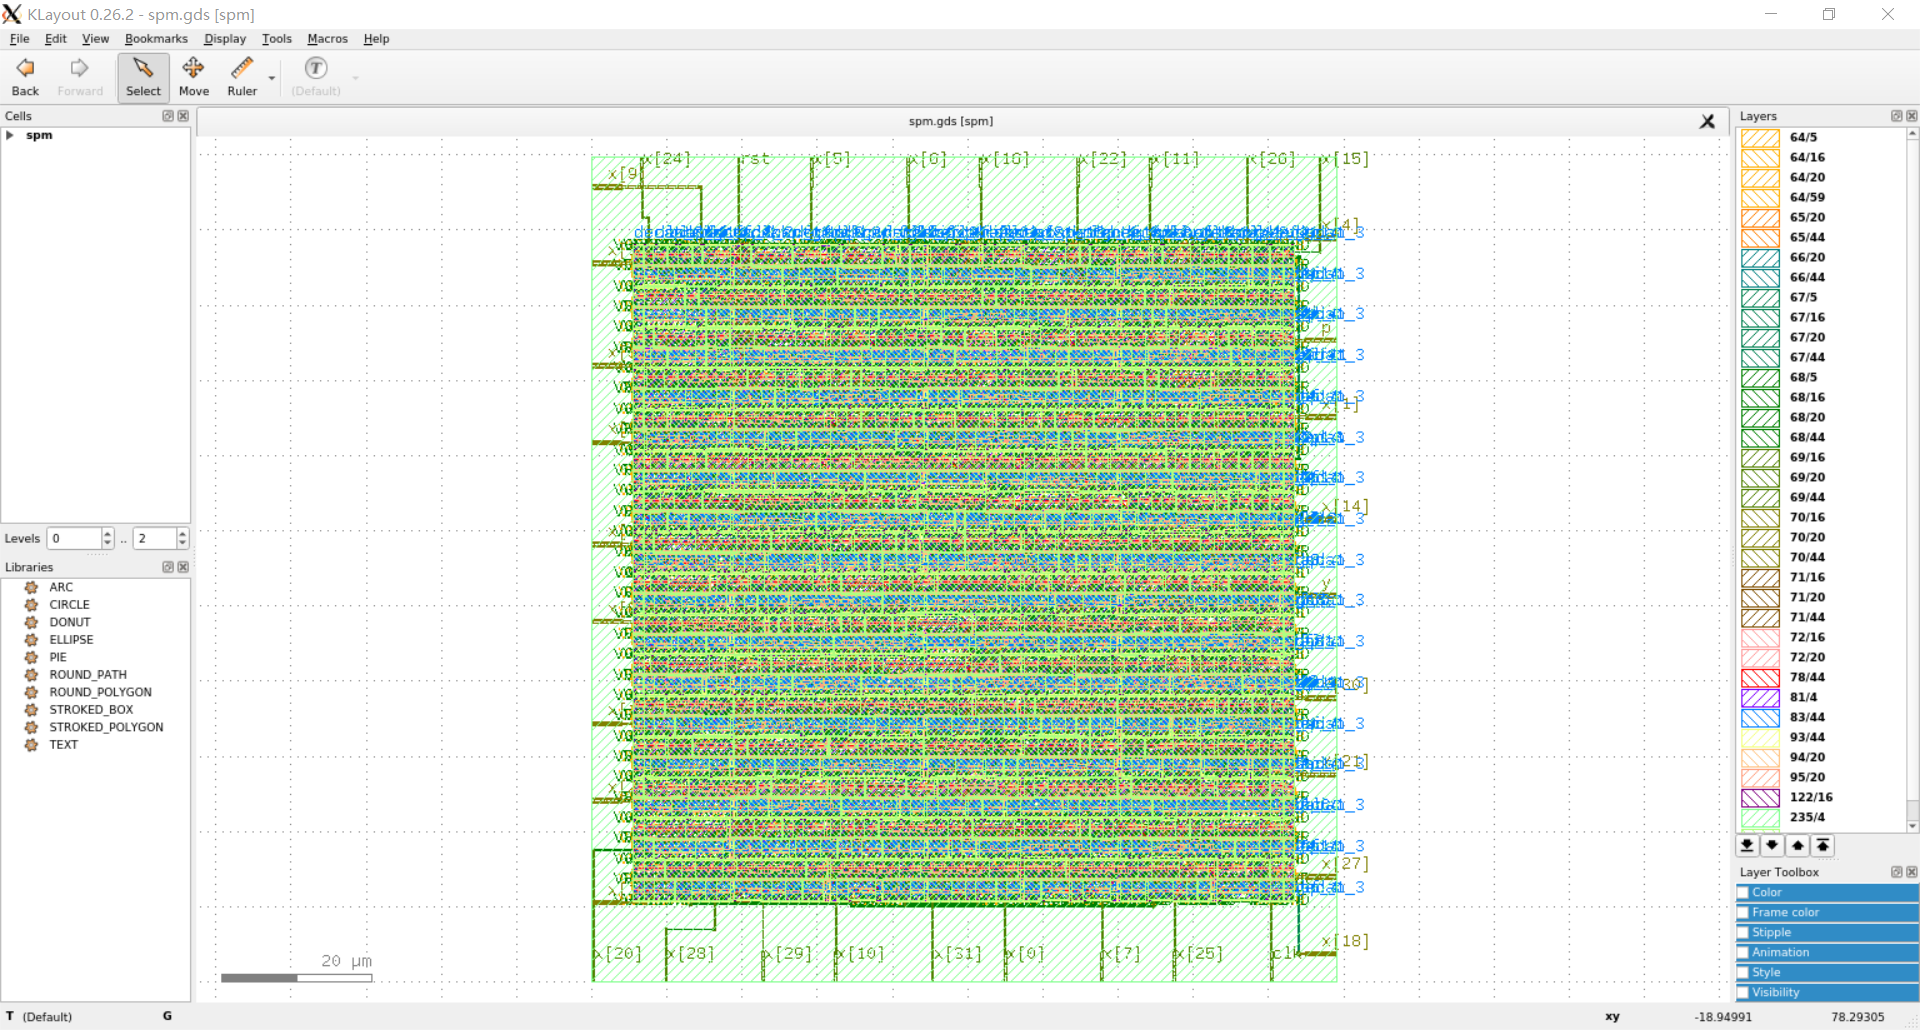
\includegraphics[width=1\textwidth]{part3_1_1.png}
    \caption{Generated layout in Klayout editer.}
\end{figure}
For "spm.gdc" in "Klayout" folder:
\begin{figure}[H]
    \centering
    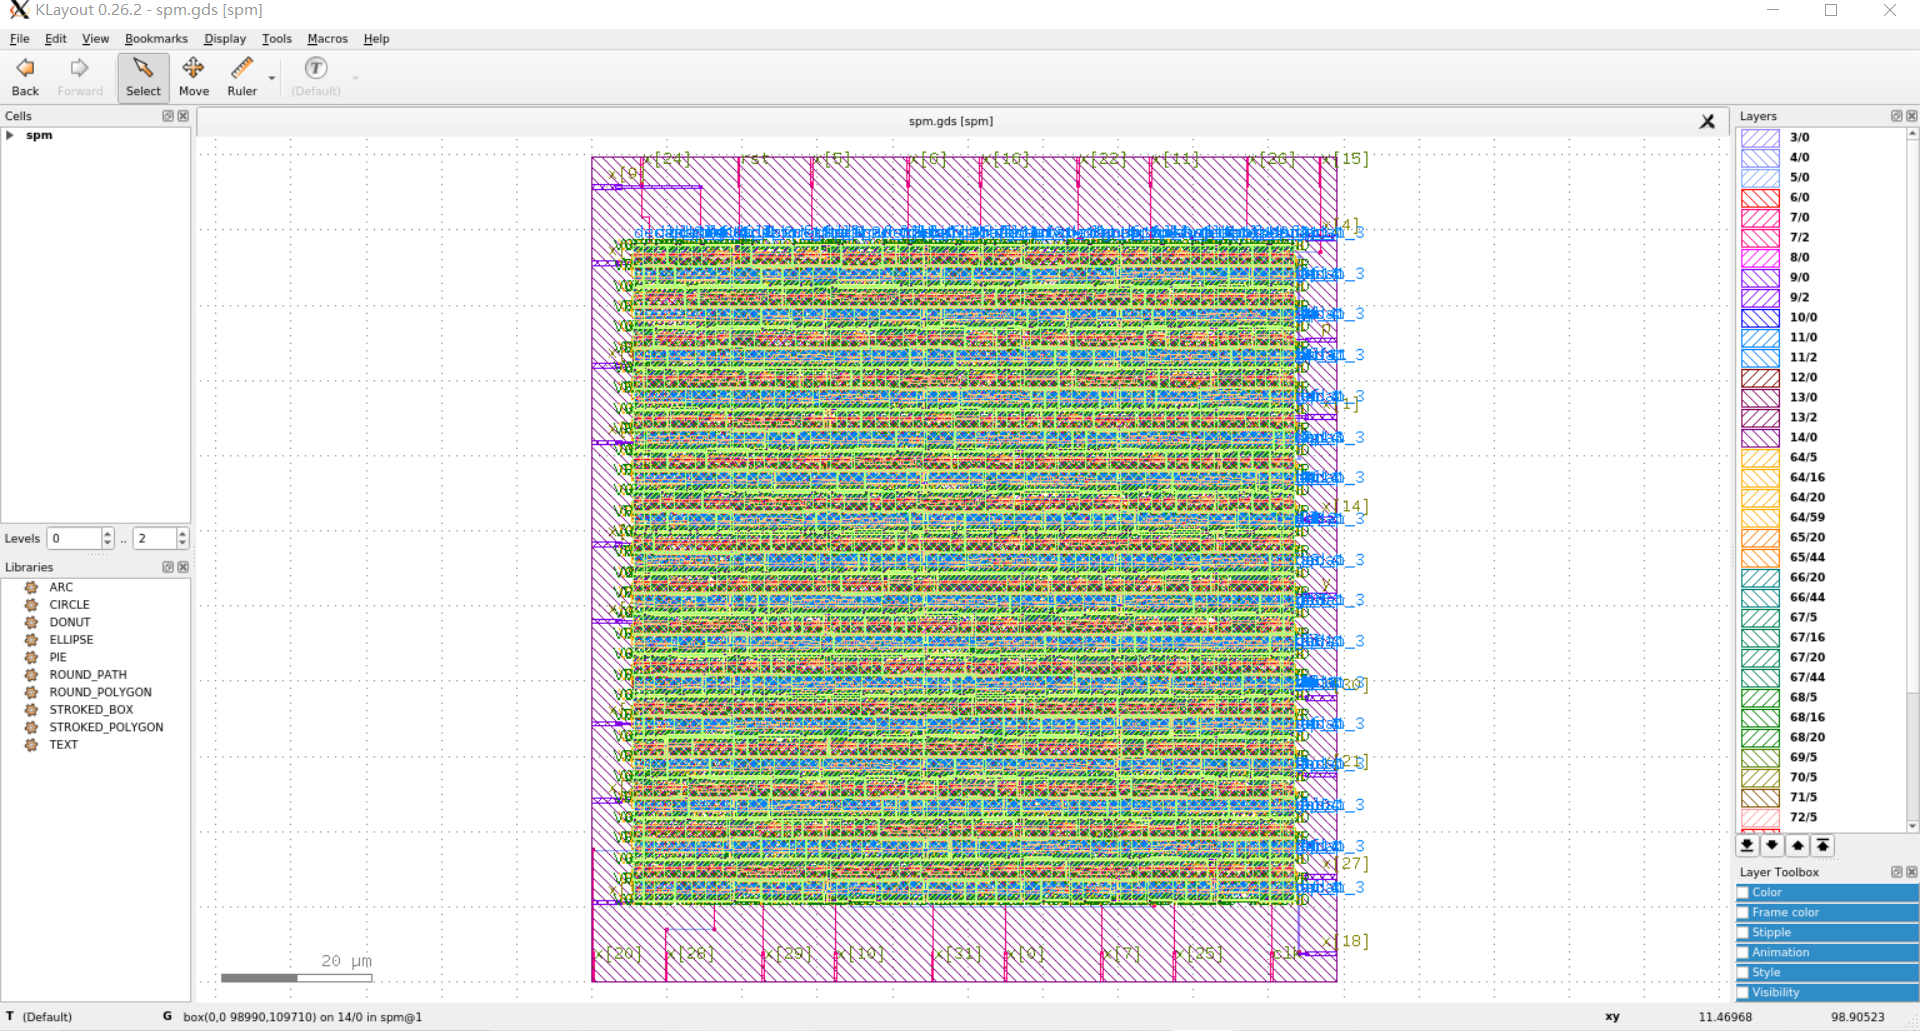
\includegraphics[width=1\textwidth]{part3_1_2.png}
    \caption{Generated layout in Klayout editer.}
\end{figure}

\subsection{Adding a Design(3.5 in lab manual)}
In this section, Verilog files provided on Canvas are added into the design in OpenLane and \\

Exercises about timing after synthesis and route: \\

1. Please modify the sdc file and create a case where setup time didn’t pass, then use the critical as an example and describe how you can fix the timing for that path. Please upload the full timing path and also your answers for fixing the timing violation.
Setup time failure:
\begin{figure}[H]
    \centering
    \includegraphics[width=1\textwidth]{exercise_1_1.png}
    \caption{Failure timing path.}
\end{figure}
Ways to fix timing violation:

The most simple way to fix setup timing violation is to reduce the clock frequency(increase clock period), but this way also deteriorates the performance as well. Other ways including improving the design to add some buffers. 

2. Please modify the sdc file and find the maximum frequency that passes the timing check after route. Please upload the screenshot of the layout after place and route, and report area and power.

When the clock period is set to 5.5ns, the design can still go through all flows and can pass the timing check after route. \\
Layout: \\
\begin{figure}[H]
    \centering
    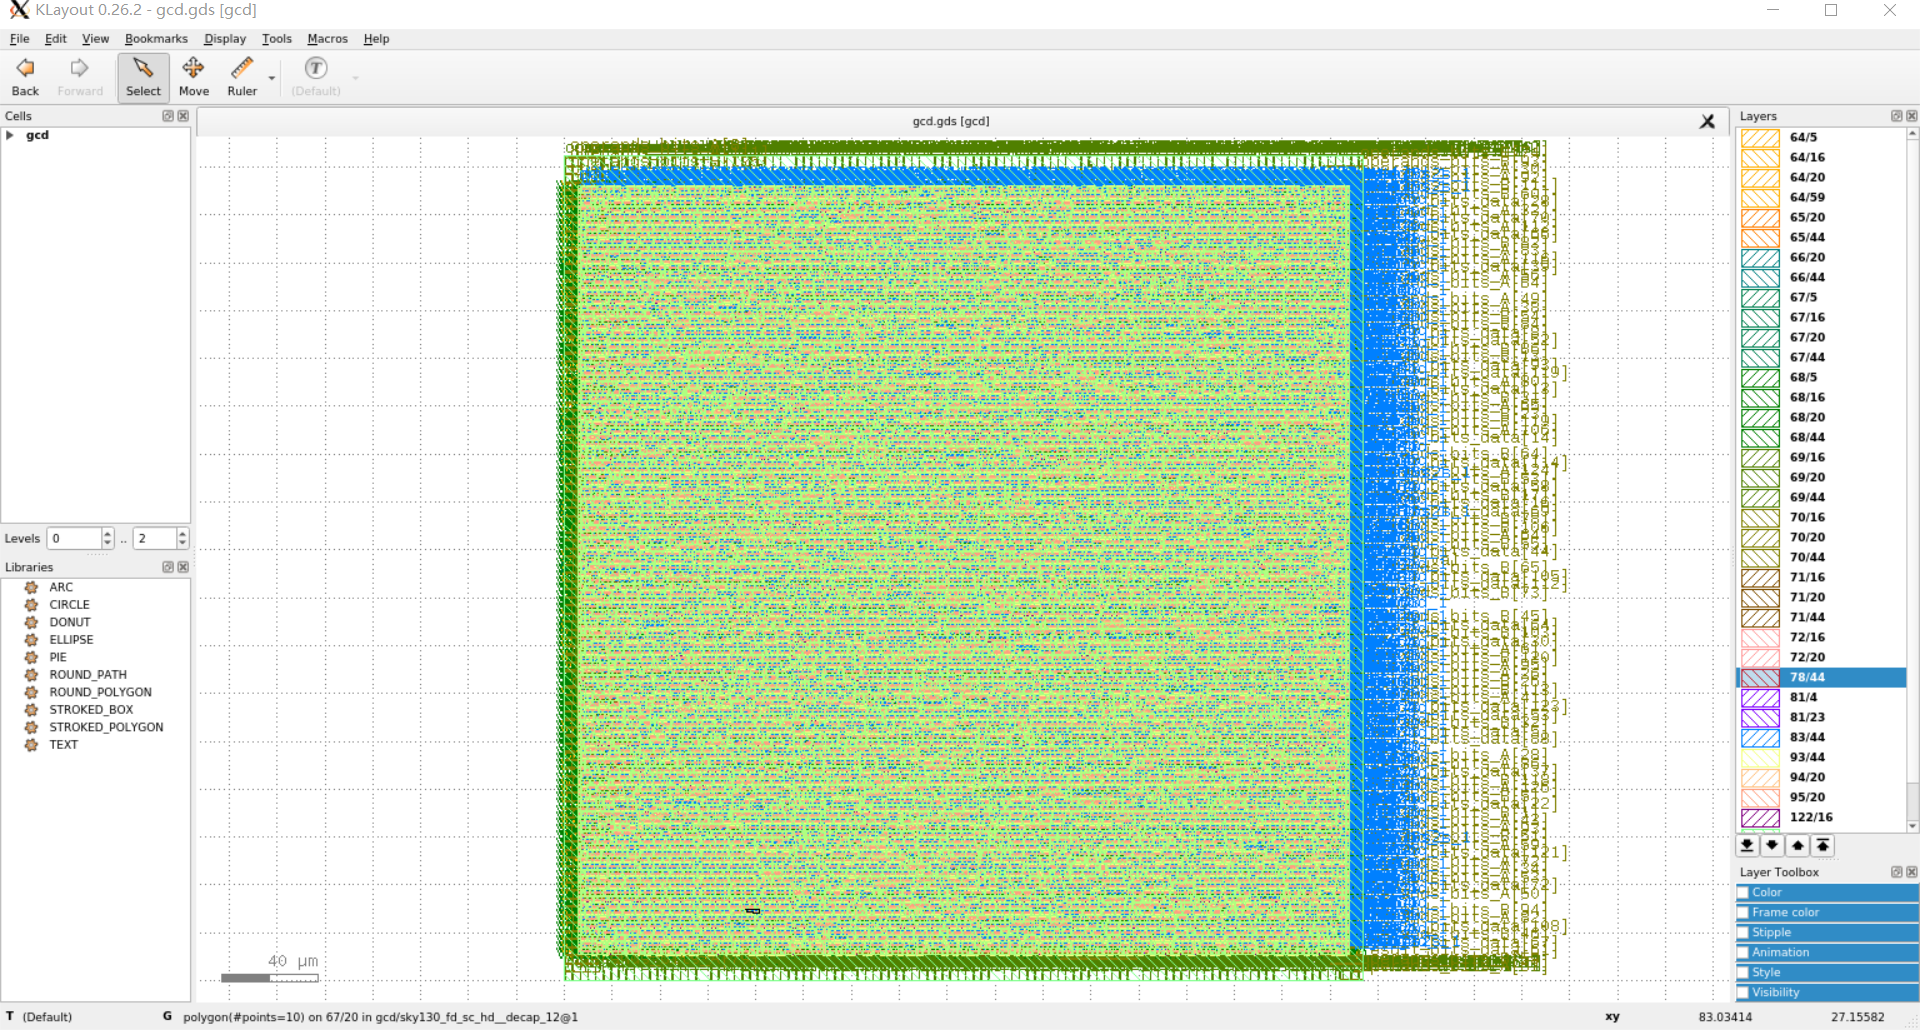
\includegraphics[width=1\textwidth]{exercise_1_2.png}
    \caption{Layout of gcd design.}
\end{figure}
Area and power: \\
\begin{figure}[H]
    \centering
    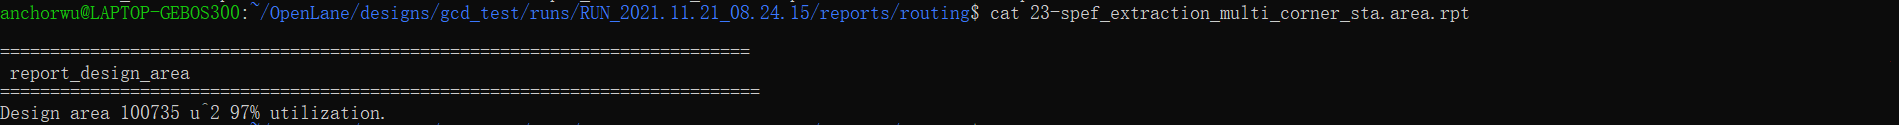
\includegraphics[width=1\textwidth]{exercise_1_2_2.png}
    \caption{Area report of gcd design.}
\end{figure}
\begin{figure}[H]
    \centering
    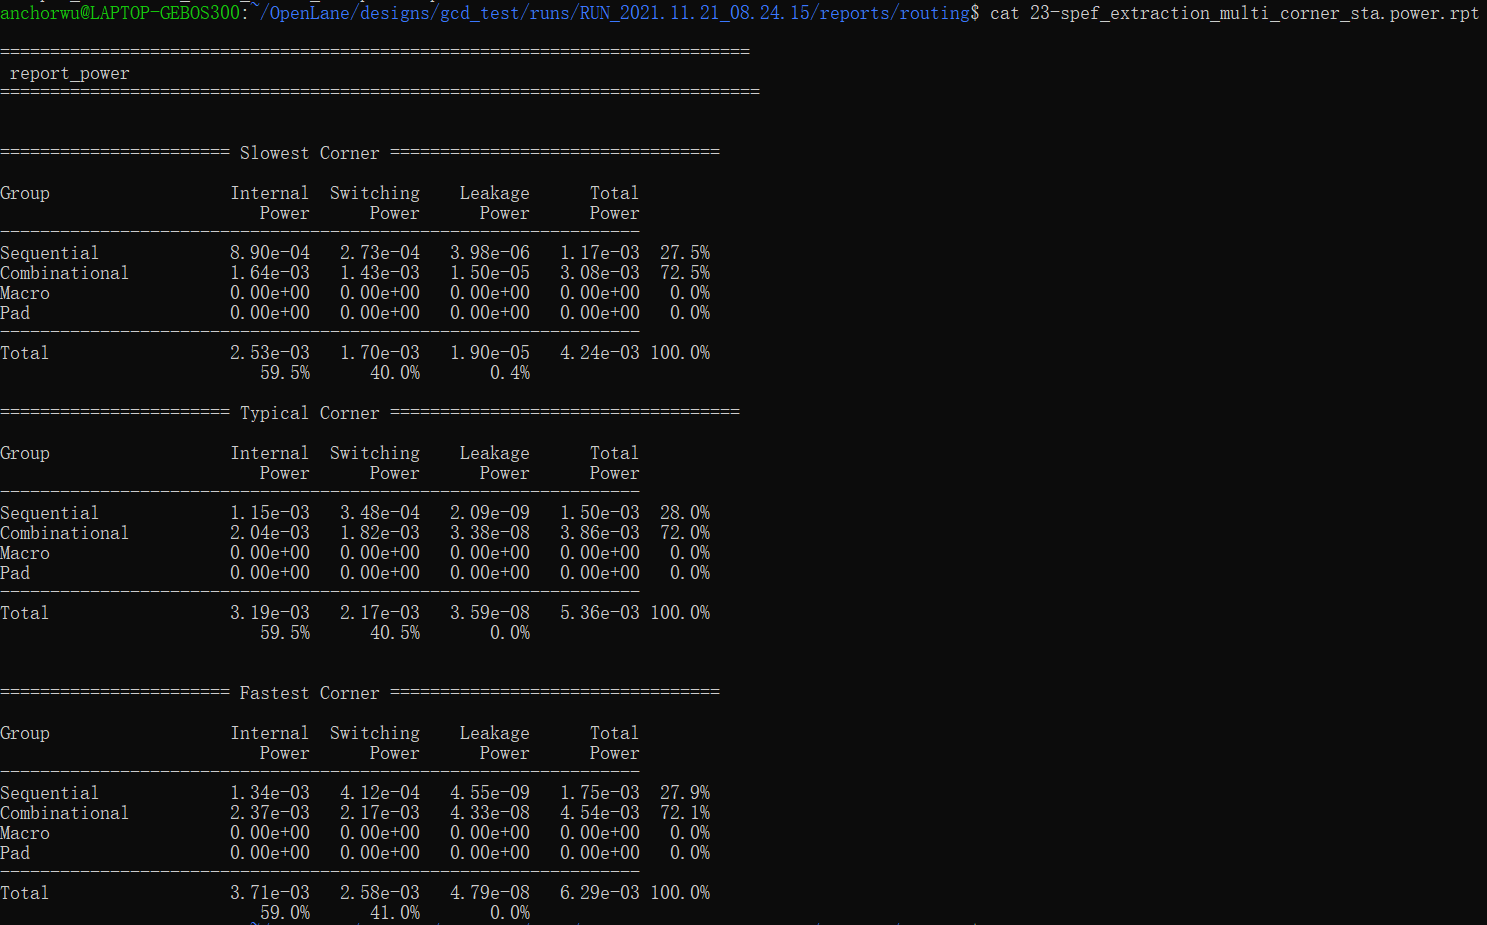
\includegraphics[width=1\textwidth]{exercise_1_2_3.png}
    \caption{Power report of gcd design.}
\end{figure}
The area is $100735um^2$ with 97\% utilization. The total power is about $4.24*10^{-3}$ w at the slowest corner, with around 59\% internal power and around 40\% switching power.

3. Please add 10\% of rise and fall time in your sdc for the clock and check the results again. Find the maximum frequency that passes the timing check. Any differences from the first experiment?\\

On previous conditions, clock period of 5.5 ns can pass through all flows. After adding 10\% of rise and fall time, 5.5ns cannot pass through all the flows and clock period of 6.0ns can pass through flows. Adding rise and fall time indeed make the timing condition harder to fulfill the requirements. 

Exercises about modifying parameters: \\
(Unless specified, all tests below are with 5.5ns clock period.)

1. Run a test where you set the core utilization target to 55\%, what did you observe? Is the flow running ok? If not, why? If so, what is the total area? How about timing?\\

In this section, I set the core utilization target to 55\% in file\\ "sky130A\_sky130\_fd\_sc\_hd\_config.tcl", instaed of original value of 25\%. I find that after this modification, the design cannot pass through the flow, because the area for floorplan is too small and there are not enough pins(as shown in figure below). 
\begin{figure}[H]
    \centering
    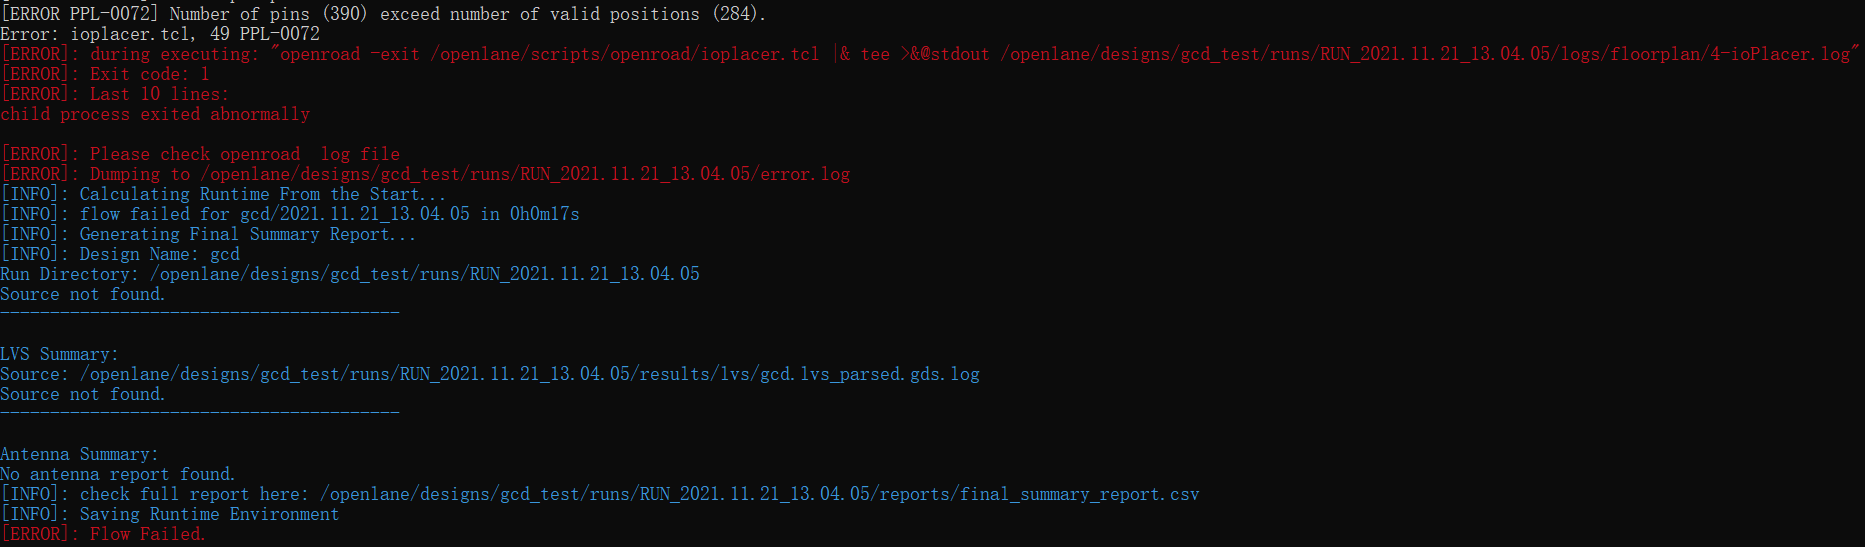
\includegraphics[width=1\textwidth]{exercise_2_1_1.png}
    \caption{Flow failed when core utilization is 55\%.}
\end{figure}
In terms of area, the die area is as the figure shown below, which is:(0, 0, 228.745, 239.465). In terms of timing, the design can still pass the 1st step of synthesis, but with several slack violations.
\begin{figure}[H]
    \centering
    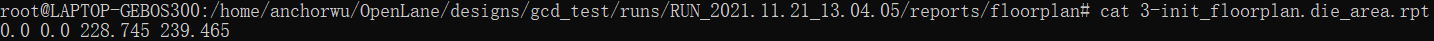
\includegraphics[width=1\textwidth]{exercise_2_1_2.png}
    \caption{Die area when core utilization is 55\%.}
\end{figure}
2. Turn on the placement timing driven and compare against a base case, any changes in timing? Please describe the timing differences.\\

By setting "set ::env(PL\_TIME\_DRIVEN) 1" in \\ "OpenLane/configuration/placement.tcl", the timing behavior becomes worse then previous cases. That's because timing driven placement will run placement mainly based on timing instead of routing.

3. Try to run synthesis at a different corner (by changing LIB\_SYNTH to a use the same lib defined by LIB\_SLOWEST. Observe if the maximum frequency and describe what you saw. How about area and power?

In this section, I change the "LIB\_SYNTH" into "LIB\_SLOWEST" in "OpenLane/scripts/synth.tcl" and "OpenLane/scripts/synth\_top.tcl"  and "OpenLane/pdks/open\_pdks/sky130/openlane/sky130\_fd\_sc\_hd/config.tcl". Then we find that this design cannot pass the flow, due to LVS errors. 
\begin{figure}[H]
    \centering
    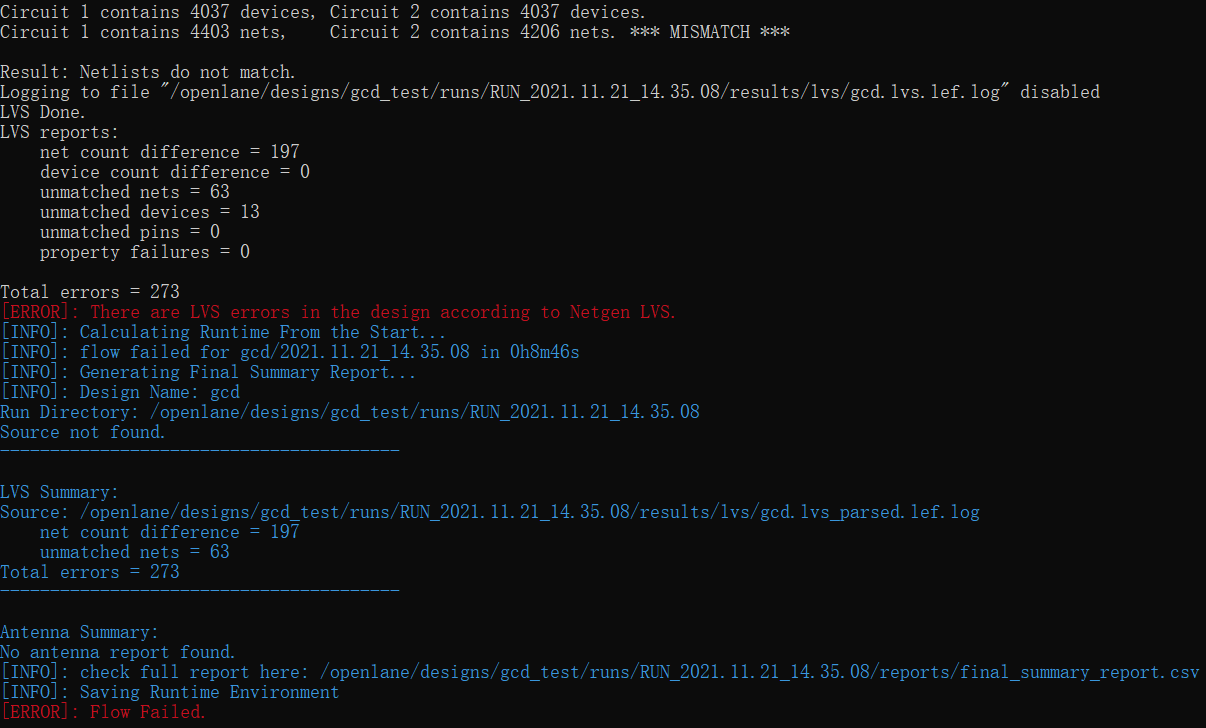
\includegraphics[width=1\textwidth]{exercise_2_3_1.png}
    \caption{Flow failure after changing corners.}
\end{figure}

4. Change CTS\_TARGET\_SKEW to 150ps (instead of 200ps), observe the timing differences, and describe your observation. Can you explain why?

As explained later, since parameter "CTS\_TARGET\_SKEW" isn't used in TritonCTS 2.0 in new version of OpenLane, and there won't be any change after varying this parameter, we just skip this exercise.

5. Change the core aspect ratio to 2:1 instead of 1:1, what did you observe, any changes about timing, area and power? Please upload the layout after changing the aspect ratio and your answers to the above question

We modify the aspect ratio in  "OpenLane/configuration/floorplan.tcl" from 1:1 to 2:1. After running through the flow, the layout becomes: 
\begin{figure}[H]
    \centering
    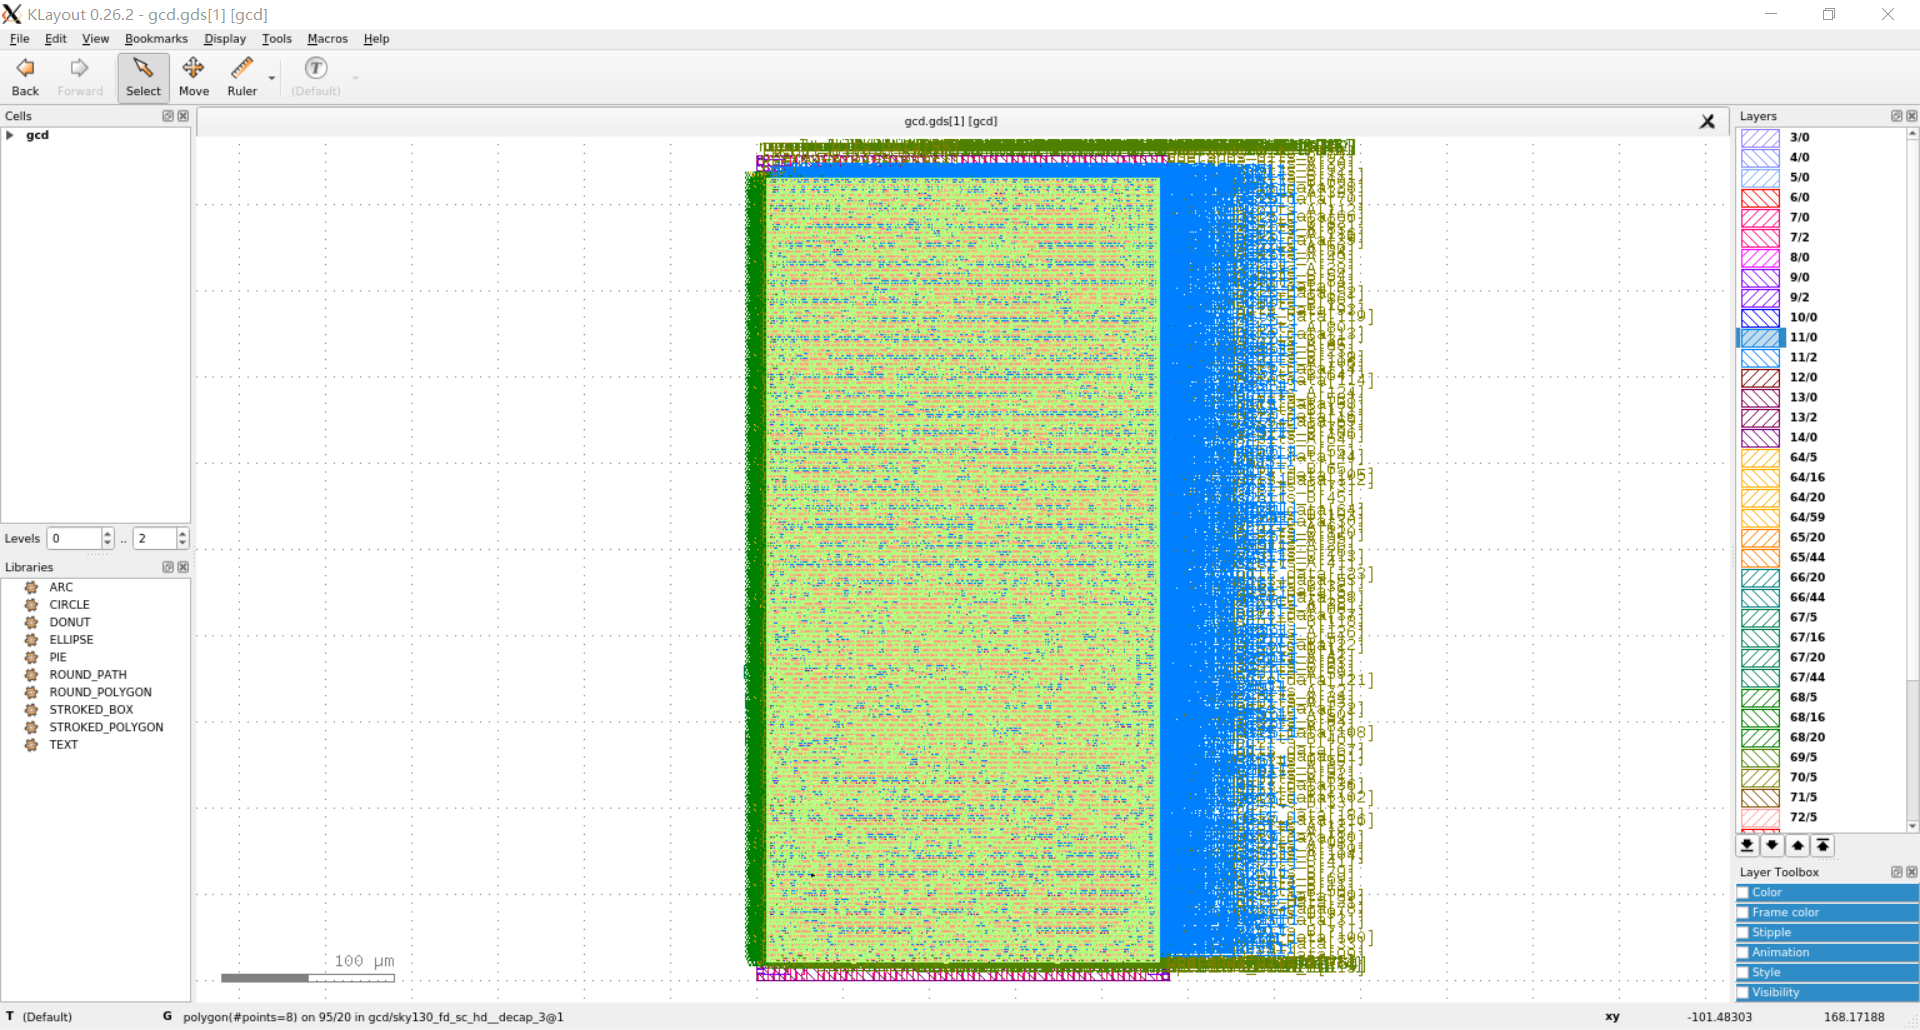
\includegraphics[width=1\textwidth]{exercise_2_5_1.png}
    \caption{Layout when aspect ratio is 2:1.}
\end{figure}
Thus, we can find that the chip area becomes a rectangular with length is two times of width. We can also find this by the area report, which becomes (0, 0, 239.37, 478.42):
\begin{figure}[H]
    \centering
    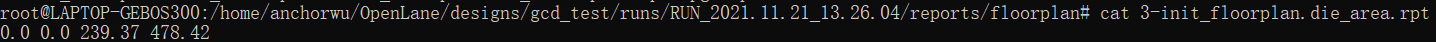
\includegraphics[width=1\textwidth]{exercise_2_5_2.png}
    \caption{Die area when aspect ratio is 2:1.}
\end{figure}

\section{Questions}
1. How many corners are in the Skywater 130nm technology libraries?\\
I find 18 ".lib" files under the folder "lib" of "sky130\_fd\_sc\_hd" in "sky130A" PDK, corresponding to 18 corners of fast-fast or slow-slow or typical-typical and also for different temperatures and threshold voltages. There are also going to be other variations of technology, such as "sky130\_fd\_sc\_hvl" etc. 
\begin{figure}[H]
    \centering
    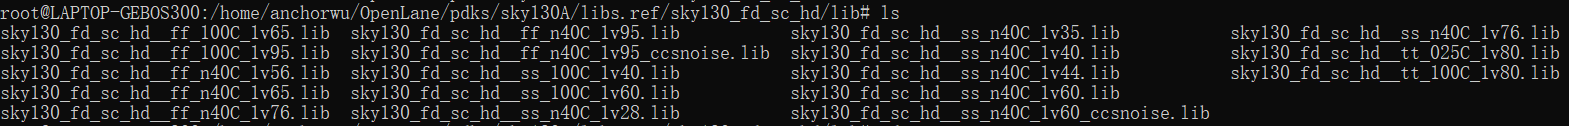
\includegraphics[width=1\textwidth]{part4_1.png}
    \caption{Corner files in "sky130\_fd\_sc\_hd".}
\end{figure}

2. In openLane, what layers are power and ground using for the power grid?

3. Is the placement and route time better or worse than synthesis timing? Why is that?

The placement and route time is worse or stricter than synthesis timing, since when some my designs can indeed pass the synthesis, they can't pass the timing check after placement and route. That's probably because even though the design can pass synthesis, there's going to be new setup/hold violations after placement and routing. If these violations can't be fixed with margin, then flow failure occurs. 

4. Why do we need to use a special buffer for clock tree? Example: in OpenLane, they used sky130\_fd\_sc\_hd\_\_clkbuf\_4.

Sometimes after synthesis there could still be some timing violations, especially after placement and routing, thus some special buffers should be inserted to fix these violations. 

5. Describe how the OpenLane project is constructed into a flow based on your observations and understanding.

OpenLane project consists of a lot of TCL scripts that run different tools. By properly configuring these scripts in a chain that processes the design with the appropriate sequential order, this flow can be generated and works. 
\end{document}
